\documentclass[a4paper,12pt]{article}

% Language and font encodings
\usepackage[english]{babel}
\usepackage[utf8x]{inputenc}
\usepackage[T1]{fontenc}

% Sets page size and margins
\usepackage[a4paper,top=3cm,bottom=2cm,left=3cm,right=3cm,marginparwidth=1.75cm]{geometry}

% Useful packages
\usepackage[fleqn]{amsmath}
\usepackage{array}
\usepackage{booktabs}
\usepackage{gensymb}
\usepackage{graphicx}
\usepackage[colorlinks=true, allcolors=blue]{hyperref}
\usepackage{makecell}
\usepackage{siunitx}
\usepackage{systeme}
\usepackage{textcomp}
\usepackage{textgreek}
\usepackage[colorinlistoftodos]{todonotes}

\title{Semestrální projekt do IEL 2016/2017}
\date{\today}
\author{Jakub Čábera <xcaber00>}

\begin{document}
\begin{titlepage}
	\centering
	{\scshape\LARGE VYSOKÉ UČENÍ TECHNICKÉ V BRNĚ \par}
	\vspace{1cm}
	{\scshape\LARGE Fakulta informačních technologií \par}
	\vspace{1.5cm}
	{\huge\bfseries Semestrální projekt do IEL 2016/2017\par}
	\vspace{2cm}
	{\Large Jakub Čábera (xcaber00)\par}
	\vfill

	% Bottom of the page
	{\large 22.12.2016 \par}
\end{titlepage}
\pagebreak

\section{Úloha 1} % DONE
	\subsection{Zadání}
		Stanovte napětí \textbf{U\textsubscript{R\textsubscript{8}}} a proud \textbf{I\textsubscript{R\textsubscript{8}}}. Použijte metodu postupného zjednodušování obvodu.
	\subsection{Tabulka hodnot}
		\begin{table}[htbp]
			\noindent\begin{tabular}{*{11}{c}}
				\toprule
				sk. & \(U_1 [V]\) & \(U_2 [V]\) & \(R_1 [\Omega]\) & \(R_2 [\Omega]\) & \(R_3 [\Omega]\) & \(R_4 [\Omega]\) & \(R_5 [\Omega]\) & \(R_6 [\Omega]\) & \(R_7 [\Omega]\) & \(R_8 [\Omega]\) \\
				\midrule
				H & 135 & 80 & 680 & 600 & 260 & 310 & 575 & 870 & 355 & 265 \\
				\bottomrule
			\end{tabular}
		\end{table}
	\subsection{Postup}
		\subsubsection{} % 1.3.1
			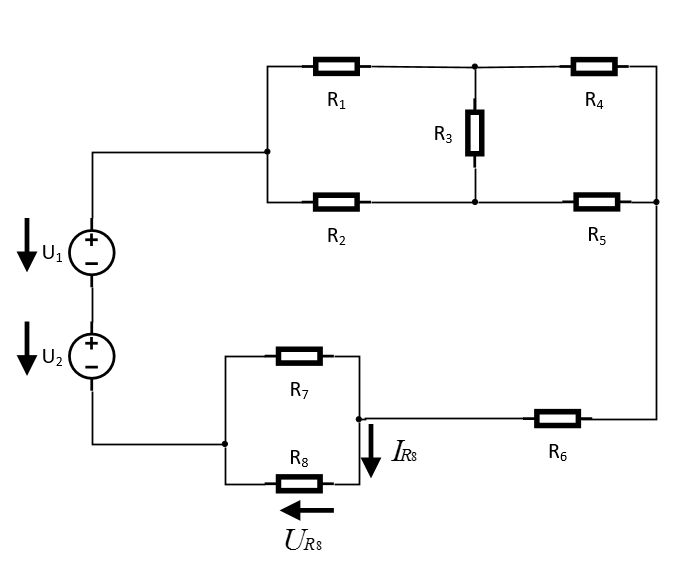
\includegraphics[width=400px]{1_1.png}
			\pagebreak
		\subsubsection{} % 1.3.2
			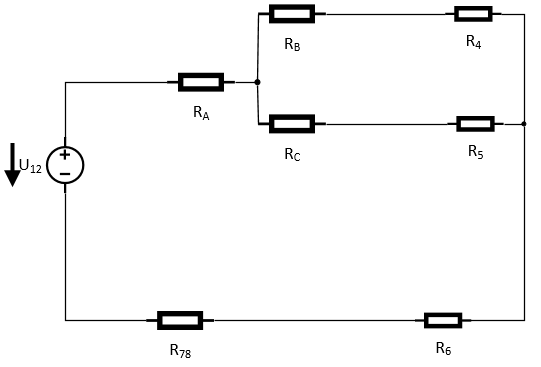
\includegraphics[width=400px]{1_2.png}
			\begin{equation}
				U_{12} = U_1 + U_2 = 215 \;[V]\nonumber
			\end{equation}
			\begin{equation}
				R_A = \frac{R_1 \times R_2}{R_1 + R_2 + R_3} = 264,9351 \;[\Omega]\nonumber
			\end{equation}
			\begin{equation}
				R_B = \frac{R_1 \times R_3}{R_1 + R_2 + R_3} = 114,8052 \;[\Omega]\nonumber
			\end{equation}
			\begin{equation}
				R_C = \frac{R_2 \times R_3}{R_1 + R_2 + R_3} = 101,2987 \;[\Omega]\nonumber
		\end{equation}
		\begin{equation}
			R_{78} = \frac{R_7 \times R_8}{R_7 + R_8} = 151,7339 \;[\Omega]\nonumber
		\end{equation}
		\subsubsection{} % 1.3.3
			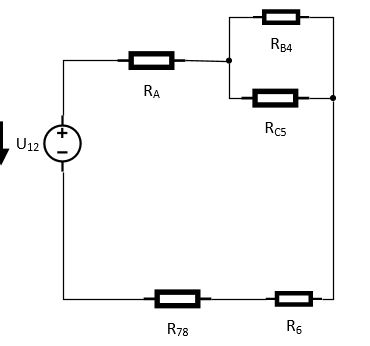
\includegraphics[width=400px]{1_3.png}
			\begin{equation}
				R_{B4} = R_B + R_4 = 4524,8052 \;[\Omega]\nonumber
			\end{equation}
			\begin{equation}
				R_{C5} = R_C + R_5 = 676,2987 \;[\Omega] \nonumber
			\end{equation}
		\subsubsection{} % 1.3.4
			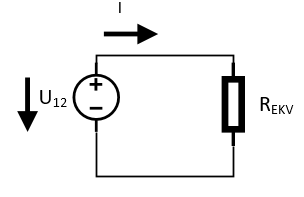
\includegraphics[width=300px]{1_4.png}
			\begin{equation}
				R_{EKV} = R_A + \frac{R_{B4} \times R_{C5}}{R_{B4} + R_{C5}} + R_6 + R_{78} = 1 547,5846 \;[\Omega]\nonumber
			\end{equation}
			\begin{equation}
				I = \frac{U_{12}}{R_{EKV}} = 0,1389 \;[A]\nonumber
			\end{equation}
		\subsubsection{} % 1.3.5
			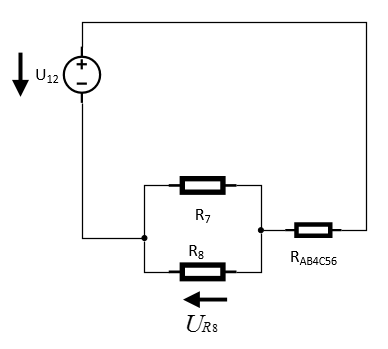
\includegraphics[width=350px]{1_5.png}
			\begin{equation}
				U_{78} = I \times R_{78} = 21,0758 \;[V] \nonumber
			\end{equation}
			\begin{equation}
				U_{78} = U_{R_7} = U_{R_8}\nonumber
			\end{equation}
			\begin{equation}
				I_{R_{8}} = \frac{U_{R_{8}}}{R_8} = 0.0795 \;[A] \nonumber
			\end{equation}
			\pagebreak
\section{Úloha 2} % DONE
	\subsection{Zadání}
		Stanovte napětí \textbf{U\textsubscript{R\textsubscript{4}}} a proud \textbf{I\textsubscript{R\textsubscript{4}}}. Použijte metodu Théveninovy věty.
	\subsection{Tabulka hodnot}
		\begin{table}[htbp]
			\centering
			\begin{tabular}{*{7}{c}}
				\toprule
				sk. & \(U [V]\) & \(R_1 [\Omega]\) & \(R_2 [\Omega]\) & \(R_3 [\Omega]\) & \(R_4 [\Omega]\) & \(R_5 [\Omega]\) \\
				\midrule
				D & 150 & 200 & 660 & 200 & 550 & 330 \\
				\bottomrule
			\end{tabular}
		\end{table}
	\subsection{Postup}
		\subsubsection{} % 2.3.1
			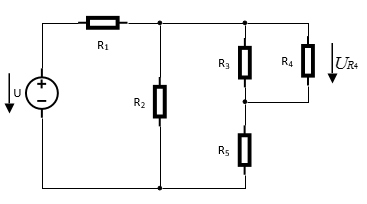
\includegraphics[width=350px]{2_1.png}
		\subsubsection{} % 2.3.2
			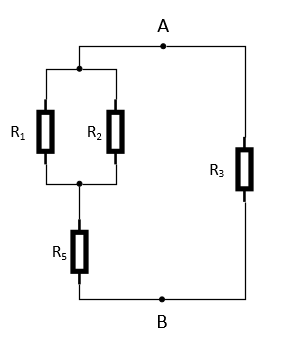
\includegraphics[width=300px]{2_3.png}
			\begin{equation}
				R_{i} = \frac{(\frac{R_1 \times R_2}{R_1 + R_2} + R_5) \times R_3}{(\frac{R_1 \times R_2}{R_1 + R_2} + R_5) + R_3} = 141,4767 \;[\Omega] \nonumber
			\end{equation}
		\subsubsection{} % 2.3.3
			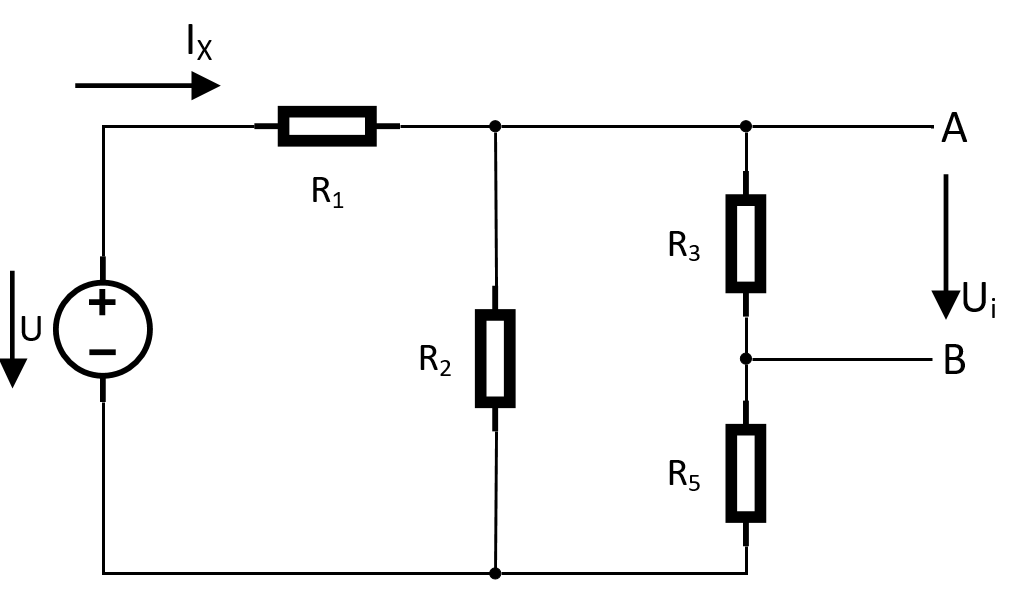
\includegraphics[width=300px]{2_2.png}
			\begin{equation}
				R_{EKV} = R1 + \frac{R_2 \times (R_3 + R_5)}{R_2 + R_3 + R_5} = 493,9496 \;[\Omega] \nonumber
			\end{equation}
			\begin{equation}
				I_X = \frac{U}{R_{EKV}} = 0,3037 \;[A] \nonumber
			\end{equation}
			\begin{equation}
				I_{R_2} = \frac{U - (I_X \times R_1)}{R_2} = 0,1488 \;[A] \nonumber
			\end{equation}
			\begin{equation}
				I_{R_{35}} = I_X - I_{R_2} = 0,1549 \;[A] \nonumber
			\end{equation}
			\begin{equation}
				U_i = U_{R_3} = I_{R_{35}} \times R_3 = 30,98 \;[V] \nonumber
			\end{equation}
		\subsubsection{}
			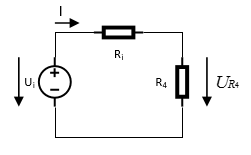
\includegraphics[width=250px]{2_4.png}
			\begin{equation}
				I = \frac{U_i}{R_i + R_4} = 0,0448 \;[A] \nonumber
			\end{equation}
			\begin{equation}
				U_{R_4} = I \times R_4 = 24,64 \;[V] \nonumber
			\end{equation}
			\begin{equation}
				I_{R_4} = \frac{U_{R_4}}{R_4} = 0,0448 \;[A] \nonumber
			\end{equation}
			\pagebreak
\section{Úloha 3} % DONE
	\subsection{Zadání}
		Stanovte napětí \textbf{U\textsubscript{R\textsubscript{4}}} a proud \textbf{I\textsubscript{R\textsubscript{4}}}. Použijte metodu uzlových napěti (U\textsubscript{A}, U\textsubscript{B}, U\textsubscript{C}).
	\subsection{Tabulka hodnot}
		\begin{table}[htbp]
			\centering
			\begin{tabular}{*{9}{c}}
				\toprule
				sk. & \(U [V]\) & \(I_1 [\Omega]\) & \(I_2 [A]\) & \(R_1 [A]\) & \(R_2 [\Omega]\) & \(R_3 [\Omega]\) & \(R_4 [\Omega]\) & \(R_5 [\Omega]\) \\
				\midrule
				A & 120 & 0,9 & 0,7 & 53 & 49 & 65 & 39 & 32 \\
				\bottomrule
			\end{tabular}
		\end{table}
	\subsection{Postup}
		\subsubsection{} % 3.3.1
			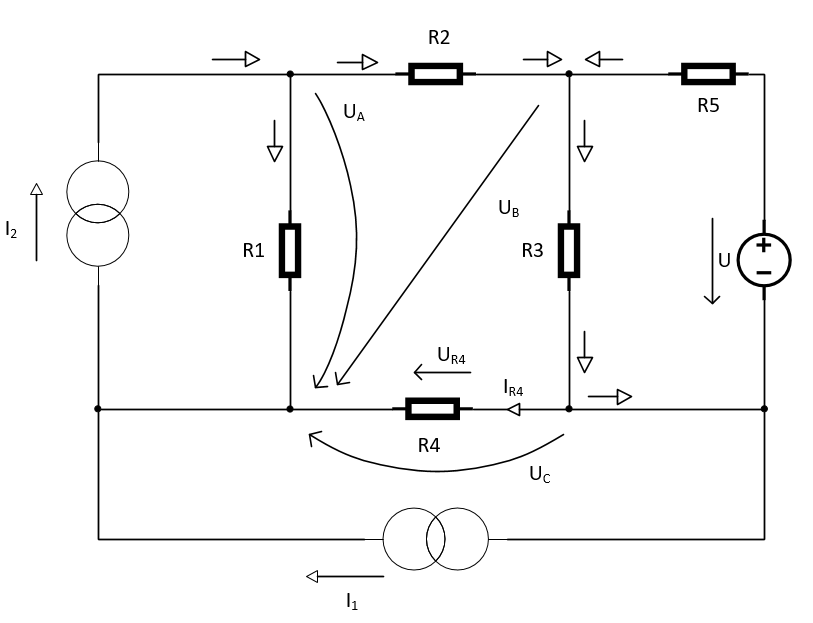
\includegraphics[width=350px]{3_1.png}
			\begin{equation}
				\mathbf{A}: I_2 - \frac{U_A}{R_1} - \frac{U_A - U_B}{R_2} = 0 \nonumber
			\end{equation}
			\begin{equation}
				\mathbf{B}: \frac{U_A - U_B}{R_2} + \frac{U - U_B + U_C}{R_5} - \frac{U_B - U_C}{R_3} = 0 \nonumber
			\end{equation}
			\begin{equation}
				\mathbf{C}: -\frac{U_C}{R_4} + \frac{U_B - U_C}{R_3} - \frac{U - U_B + U_C}{R_5} -I_1  = 0 \nonumber
			\end{equation}
		\subsubsection{} % 3.3.2
			\begin{math}
				\mathbf{A:\;} I_2 \times R_1 \times R_2 - U_A \times R_2 - U_A \times R_1 + U_B \times R_1 = 0 \\
			\end{math}
			\begin{math}
				\mathbf{B:\;} U_A \times R_5 \times R_3 - U_B \times R_5 	\times R_3 - U \times R_2 \times R_3 - U_B \times R_2 \times R_3 + U_C \times R_2 \times R_3 - U_B \times R_2 \times R_5 + U_C \times R_2 \times R_5  +1 +2 +3 +4 +5 = 0 \\
			\end{math}
			\begin{math}
				\mathbf{C:} -U_C \times R_3 \times R_5 + U_B \times R_4 \times R_5 - U_C \times R_5 \times R_4 - U \times R_4 \times R_3 - U_C \times R_4 \times R_3 - I_1 \times R_4 \times R_3 \times R_5 = 0 \\
			\end{math}
			\begin{math}
				\mathbf{A:\;} U_A \times (-R_2 -R_1) + U_B \times R_1  + 0 \times U_C = -I_2 \times R_1 \times R_2 \\
			\end{math}
			\begin{math}
				\mathbf{B:\;} U_A \times (R_5 \times R_3) + U_B \times (-R_5 \times R_3 - R_2 \times R_3 - R_2 \times R_5) + U_C \times (R_2 \times R_3 + R_2 \times R_5) = -U \times R_2 \times R_3 \\
			\end{math}
			\begin{math}
				\mathbf{C:\;} 0 \times R_A + U_B \times (R_4 \times R_5 + R_4 \times R_3) + U_C \times (-R_3 \times R_5 - R_4 \times R_5 - R_4 \times R_3) = U \times R_4 \times R_3 + I_1 \times R_4 \times R_3 \times R_5 \\
			\end{math}
			\begin{equation}
				M_0 = \begin{pmatrix}
					-102 & 53 & 0 \\
					2080 & -6833 & 4753 \\
					0 & 3783 & -5863
				\end{pmatrix} \nonumber
			\end{equation}
			\begin{math}
				M_0 = [(-102) \times (-6833) \times (-5863) + 2080 \times 3783 \times 0 + 0 \times 53 \times 4753] - [(-6833) \times 0 \times 0 + 4753 \times 3783 \times (-102) + (-5863) \times 53 \times 2080] = \mathbf{-1 605 953 440} \nonumber
			\end{math} \\
			\begin{equation}
				M_1 = \begin{pmatrix}
					-102 & 53 & -1817,9 \\
					2080 & -6833 & -382 200 \\
					0 & 3783 & 377 208
				\end{pmatrix} \nonumber
			\end{equation}
			\begin{math}
				M_1 = [(-102) \times (-6833) \times 377208 + 2080 \times 3783 \times (-1817,9) + 0 \times 53 \times (-382200)] - [(-6833) \times 0 \times (-1817,9) + (-382200) \times 3783 \times (-102) + 377208 \times 53 \times 2080] = \mathbf{59 535 355 152} \nonumber
			\end{math} \\
			\begin{equation}
				U_{R_4} = U_C = \frac{\det(M_1)}{\det(M_0)} = -37,0717 \;[V]\nonumber
			\end{equation}
			\begin{equation}
				I_{R_4} = \frac{U_{R_4}}{R_4} = -0,9506 \;[A] \nonumber
			\end{equation}
			\pagebreak
\section{Úloha 4} % DONE
	\subsection{Zadání} % DONE
		Pro napájecí napětí platí: \(u_1 = U_1 \times \sin (2\pi ft), u_2 = U_2 \times \sin (2\pi ft)\).
		Ve vztahu pro napětí \(u_{C_1} = U_{C_1} \times \sin (2 \pi ft)\) určete \textbf{|\(U_{C_1}\)| a \(\varphi_{C_1}\).} Použijte metodu smyčkových proudů.
	\subsection{Tabulka hodnot} % DONE
		\begin{table}[htbp]
			\centering
				\begin{tabular}{*{11}{c}}
					\toprule
					sk. & U\textsubscript{1} [V] & U\textsubscript{2} [V] & R\textsubscript{1} [\textOmega] & R\textsubscript{2} [\textOmega] & R\textsubscript{3} [\textOmega] & L\textsubscript{1} [mH] & L\textsubscript{2} [mH] & C\textsubscript{1} [µF] & C\textsubscript{2} [µF] & f [Hz] \\
					\midrule
					H & 65  & 60 & 10 & 10 & 12 & 160 & 75 & 155 & 70 & 95 \\
					\bottomrule
			   \end{tabular}
		\end{table}
	\subsection{Postup}
		\subsubsection{} % 4.3.1
			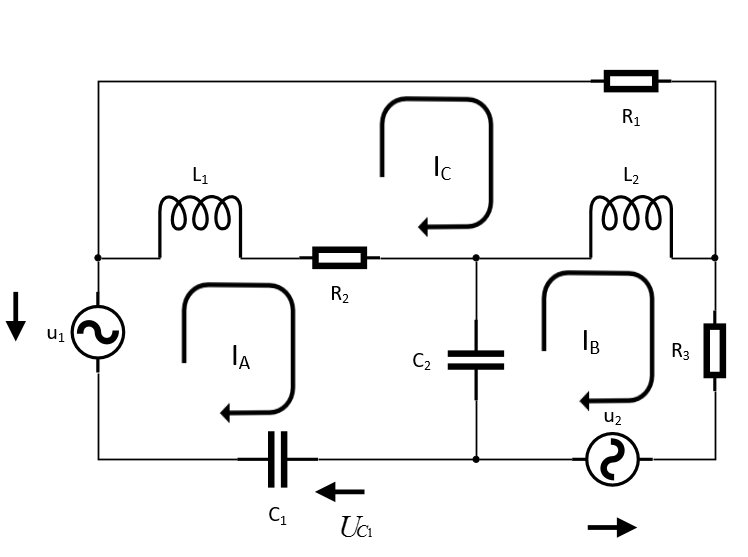
\includegraphics[width=350px]{4_1.png} \\
				\(X_{R_1} = R_1 = 10 \;[\Omega]\) \\
				\(X_{R_2} = R_2 = 10 \;[\Omega]\) \\
				\(X_{R_3} = R_3 = 12 \;[\Omega]\) \\
				\(w = 2 \pi f = 596,9026 \;[\frac{rad}{s}]\) \\
				\(X_{L_1} = jwL_1 = j95,504 \;[\Omega]\) \\
				\(X_{L_2} = jwL_2 = j44,7677 \;[\Omega]\) \\
				\(X_{C_1} = \frac{1}{jwC_1} = -j12.8351 \;[\Omega]\) \\
				\(X_{C_2} = \frac{1}{jwC_2} = -j28.4205 \;[\Omega]\) \\
			\pagebreak \\
			\begin{math}
				\mathbf{I_A:\;} X_{L_1} \times (I_A - I_C) + X_{R_2} \times (I_A - I_C) + X_{C_2} \times (I_A - I_B) + X_{C_1} \times I_A - U_1 = 0 \nonumber \\
			\end{math}
			\begin{math}
				\mathbf{I_B:\;} X_{L_2} \times (I_B - I_C) + X_{R_3} \times I_B - U_2 + X_{C_2} \times (I_B - I_A) = 0 \nonumber \\
			 \end{math}
			\begin{math}
				\mathbf{I_C:\;} X_{R_1} \times I_C + X_{L_2} \times (I_C - I_B) + X_{R_2} \times (I_C - I_A) + X_{L_1} \times (I_C - I_A) = 0 \nonumber \\
			\end{math}
			\begin{math}
				\mathbf{I_A:\;} I_A \times (X_{L_1} + X_{R_2} + X_{C_2} + X_{C_1}) -I_B \times X_{C_2} + I_C \times (-X_{L_1} - X_{R_2}) = U_1 \nonumber \\
			\end{math}
			\begin{math}
				\mathbf{I_B:} -I_A \times X_{C_2} + I_B \times (X_{L_2} + X_{R_3} + X_{C_2}) - I_C \times X_{L_2} = U_2 \nonumber \\
			\end{math}
			\begin{math}
				\mathbf{I_C:\;} I_A \times (-X_{R_2} -X_{L_1}) - I_B 	\times X_{L_2} + I_C \times (X_{R_1} + X_{L_2} + X_{R_2} + X_{L_1}) = 0 \nonumber \\
			\end{math}
			\begin{math}
				\mathbf{I_A:\;} I_A \times (10 + j54,2484) + I_B \times (j28,4205) + I_C \times (-10 - j95,504) = 65 \nonumber \\
			\end{math}
			\begin{math}
				\mathbf{I_B:\;} I_A \times (j28,4205) + I_B \times (12 + j16,3472) + I_C \times (-j44,7677) = 60 \nonumber \\
			\end{math}
			\begin{math}
				\mathbf{I_C:\;} I_A \times (-10 -j95,504) + I_B \times (-j44,7677) + I_C \times (20 + j140,2717) = 0 \nonumber \\
			\end{math}
			\begin{equation}
				M_0 = \begin{pmatrix}
					  10 + j54,2484 & j28,4205 & -10 - j95,504 \\
					  j28,4205 & 12 + j16,3472 & -j44,7677 \\
					  -10 -j95,504 & -j44,7677 & 20 + j140,2717
				\end{pmatrix} \nonumber
			\end{equation}
			%====================================================
			\begin{equation}
				M_0 = \begin{pmatrix}
					65 & j28,4205 & -10 - j95,504 \\
					60 & 12 + j16,3472 & -j44,7677 \\
					0 & -j44,7677 & 20 + j140,2717
				\end{pmatrix} \nonumber
			\end{equation}
			\begin{equation}
				I_A = \frac{\det(M_1)}{\det(M_0)} = 137.936 -j53.7687 \;[A] \nonumber
			\end{equation}
			\begin{equation}
				U_{C_1} = I_A \times X_{C_1} = 148,045 \;[V] \nonumber %sPATNE
			\end{equation}
			\begin{equation}
				\varphi_{C_1} =  -21,2963 \;[\degree C] \nonumber
			\end{equation}
			\pagebreak
\section{Úloha 5}
	\subsection{Zadání} % DONE
		Sestavte deferenciální rovnici popisující chování obvodu na obrázku, dále ji upravte dosazením hodnot parametrů. Vypočítejte analytické řešení \(i_L = f(t)\).
		Proveďte kontrolu výpočtu dosazením do sestavené diferenciální rovnice.
	\subsection{Tabulka hodnot} % DONE
		\begin{table}[htbp]
			\centering
				\begin{tabular}{*{5}{c}}
					\toprule
					sk. & \(U [V]\) & \(L [H]\) & \(R [\Omega]\) & \(i_L(0) [A]\) \\
					\midrule
					D & 5 & 50 & 40 & 2 \\
					\bottomrule
			\end{tabular}
		\end{table}
	\subsection{Postup} % TODO:
		\subsubsection{}
			TODO
		\subsubsection{}
			TODO
		\subsubsection{}
			TODO
\section{Výsledná tabulka}
	\begin{table}[htbp]
		\centering\noindent\begin{tabular}{*{2}{c}}
			\toprule
			Úloha & Výsledek \\
			\midrule
			1 & \makecell{\({U_R}_8 = 21,0758 \;[V]\) \\
						\({I_R}_8 = 0,0795 \;[A]\)}  \\
			\midrule
			2 & \makecell{\({U_R}_4 = 24,64 \;[V]\) \\
						\({I_R}_4 = 0,0448 \;[A]\)}  \\
			\midrule
			3 & \makecell{\({U_R}_4 = −37,0717 \;[V]\) \\
						\({I_R}_4 = −0,9506 \;[A]\) \\} \\
			\midrule
			4 & \makecell{\(|U_{C_1}| = 148,045 \;[V]\) \\
						\(\varphi_{C_1} = −21,2963 \;[\degree C] \)} \\
			\midrule
			5 & TODO \\
			\bottomrule
		\end{tabular}
	\end{table}

\end{document}
